\documentclass[conference]{IEEEtran}
\IEEEoverridecommandlockouts

\usepackage{cite}
\usepackage{amsmath,amssymb,amsfonts}
\usepackage{algorithmic}
\usepackage{graphicx}
\usepackage{textcomp}
\usepackage{xcolor}
\usepackage{booktabs}
\usepackage{multirow}
\usepackage{url}
\usepackage[hidelinks]{hyperref}

\def\BibTeX{{\rm B\kern-.05em{\sc i\kern-.025em b}\kern-.08em
    T\kern-.1667em\lower.7ex\hbox{E}\kern-.125emX}}

\begin{document}

\title{A Contactless Wellness Pipeline with a Controlled Study of\\
Cross-Modal HRV Adaptation for Stress Detection}

\author{
\IEEEauthorblockN{[Author Name]}
\IEEEauthorblockA{\textit{[Department]}\\
\textit{[University]}, [City, Country]\\
[email]}
}

\maketitle

\begin{abstract}
Contactless physiological monitoring via remote photoplethysmography
(rPPG) promises scalable wellness assessment from a single camera. A
common assumption in the contactless stress detection literature is
that stress classifiers trained on contact-sensor data can be adapted
to rPPG data through domain alignment. We test this assumption and
find it fails in a specific, measurable way.

We present a contactless pipeline estimating heart rate (HR), heart
rate variability (HRV), stress, and emotion from facial video. On 42
UBFC-rPPG subjects the pipeline achieves 2.71 bpm HR MAE against
finger PPG using quality-weighted ROI fusion of POS signals, without
any learned components. On a 3-class valence subset of AffectNet
(7{,}797 images), an EfficientNet-B0 head reaches 0.74 accuracy.

We then study HRV-based cross-modal adaptation. We measure the
rPPG-specific HRV feature error on UBFC (finger PPG vs.\ rPPG, same
subjects, same clips), retaining six features with median relative
error below 32\%. Using these features we build a synthetic-rPPG
version of WESAD by applying the measured noise model to chest-ECG
features, then evaluate five stress-classification configurations
under subject-independent 5-fold cross-validation with per-subject
Wilcoxon tests ($n{=}15$).

Our central finding is that adaptation is not the obstacle: chest-ECG
features are simply more stress-discriminative than wrist-PPG features
recorded on the same subjects (binary macro-F1 $0.759$ vs.\ $0.646$;
3-class $0.457$ vs.\ $0.340$). Aligning toward the less discriminative
modality monotonically degrades performance (binary $0.627$, 3-class
$0.401$), and this pattern is consistent across both task difficulties.
We report this as an observation about modality-specific
discriminability, without claims about the broader failure of domain
adaptation. Code and cached features are released for reproducibility.
\end{abstract}

\begin{IEEEkeywords}
remote photoplethysmography, heart rate variability, stress detection,
contactless sensing, domain adaptation
\end{IEEEkeywords}

% ======================================================================
\section{Introduction}

Contactless measurement of physiological state from facial video has
advanced rapidly over the past decade. Remote photoplethysmography
(rPPG) now reliably recovers heart rate (HR) from a webcam under
controlled conditions~\cite{verkruysse2008, dehaan2013, wang2017}, and
a growing literature addresses heart rate variability
(HRV)~\cite{mcduff2017, yan2019} and affective
state~\cite{meziati2021} from the same signal. The appeal is
practical: no wearable, no contact electrodes, no session setup.

Deployment of a contactless stress classifier, however, faces a data
scarcity problem. Large labeled corpora exist for contact stress
sensing --- WESAD~\cite{schmidt2018}, DEAP~\cite{koelstra2012} --- but
these datasets contain no video. Contactless datasets with matched
stress labels are rare. A natural workaround is to train on labeled
contact features and adapt the classifier to the rPPG feature space
via domain alignment. This is a common assumption in the field, but it
has not, to our knowledge, been tested in a setting where the
alignment target matches the deployment distribution.

\subsection{Contributions}

This paper makes four contributions:

\begin{enumerate}
\item \textbf{A contactless pipeline} with HR, HRV, stress, and emotion
modules. HR is validated at 2.71 bpm MAE on 42 UBFC subjects without
any learned components. Emotion reaches 0.74 accuracy on a 3-class
AffectNet subset.

\item \textbf{A controlled measurement of rPPG-specific HRV feature
error.} Finger PPG and rPPG are recorded simultaneously on the same
UBFC clips. We report per-feature deviation and identify six HRV
features that survive rPPG extraction (median relative error
$<32\%$) and four that do not ($>50\%$).

\item \textbf{A discriminability comparison between contact
modalities.} On WESAD, chest-ECG HRV features are more
stress-discriminative than wrist-PPG features recorded on the same
subjects under the same protocol.

\item \textbf{A negative result on covariance alignment.} Aligning
ECG features toward PPG features, and further toward synthetic rPPG
features, degrades stress classification monotonically on both binary
and 3-class tasks. We attribute this to the modality-specific
discriminability gap, not to a general failure of domain adaptation.
\end{enumerate}

The last point is the paper's main finding. It is presented as a
measured observation, not as a claim about the field.

% ======================================================================
\section{Related Work}

\subsection{rPPG signal extraction}
Verkruysse et al.~\cite{verkruysse2008} first demonstrated
camera-based pulse recovery. Colour-space methods followed: CHROM
\cite{dehaan2013} cancels specular reflection by combining
chrominance channels; POS~\cite{wang2017} projects normalized RGB onto
a plane orthogonal to the skin-tone direction. Deep approaches
(DeepPhys, PhysNet, MTTS-CAN, EfficientPhys) improve accuracy on
controlled benchmarks but require large labelled corpora. This work
uses POS with quality-weighted ROI fusion; no learned model is
involved in HR extraction.

\subsection{HRV from rPPG}
HRV features are more sensitive to rPPG noise than HR itself. McDuff
et al.~\cite{mcduff2017} and Yan et al.~\cite{yan2019} characterize
this gap across pipelines. UBFC-Phys~\cite{meziati2021} provides
stress-labelled video with matched physiological signals, but is
otherwise unique. We contribute a direct per-feature measurement on
UBFC, which has simultaneous finger PPG and rPPG on identical clips.

\subsection{Stress classification from HRV}
Time-domain markers (RMSSD, SDNN, pNN50) and frequency-domain markers
(LF/HF) are standard. WESAD~\cite{schmidt2018} is the reference corpus
for contact stress detection. Published subject-independent binary
results on WESAD range from $0.75$ to $0.88$ macro-F1; our
source-only baseline at $0.759$ is within that band.

\subsection{Cross-modal domain adaptation}
Deep CORAL~\cite{sun2016}, DANN~\cite{ganin2016}, and MMD-based
methods are widely applied in computer vision. Their use for HRV
transfer between sensing modalities is less explored. This work
evaluates CORAL on a calibrated synthetic target and reports a
negative result.

% ======================================================================
\section{Methodology}

\subsection{Pipeline overview}
The full pipeline is shown in Fig.~\ref{fig:pipeline}. Given a face
video at $f_s$ fps, the system produces $\{\widehat{\mathrm{HR}},
\widehat{\mathrm{HRV}}, \hat{s}, \hat{e}\}$ where $\hat{s}$ is a
stress class and $\hat{e}$ is a valence class. The modules are
independent; this is not a shared-backbone multi-task network.

\begin{figure}[t]
\centering
%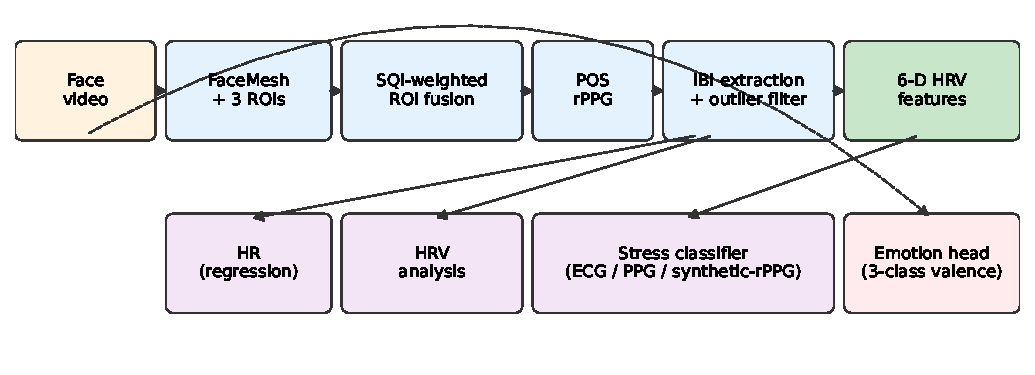
\includegraphics[width=\columnwidth]{figures/pipeline.pdf}
\caption{Contactless wellness pipeline. Face video is processed
through ROI extraction, quality-weighted fusion, and POS to obtain
inter-beat intervals. Six HRV features feed three downstream heads:
HR regression, HRV analysis, and stress classification. Emotion is
predicted from a separate face-image branch.}
\label{fig:pipeline}
\end{figure}

\subsection{ROI extraction and quality-weighted fusion}
Facial landmarks are detected with MediaPipe FaceMesh (468 points).
Three rectangular ROIs are placed on the landmark bounding box:
forehead, left cheek, right cheek. For each ROI $r$ and frame $t$ the
spatial mean RGB is computed, giving $\mathbf{c}_r(t)$.

A per-ROI Signal Quality Index combines spectral concentration in
$[0.7,4.0]$~Hz with the prominence of the autocorrelation peak. Fusion
weights are proportional to these indices:
\begin{equation}
w_r = \frac{\mathrm{SQI}_r}{\sum_{r'} \mathrm{SQI}_{r'}}, \qquad
\mathbf{c}(t) = \sum_r w_r \, \mathbf{c}_r(t).
\end{equation}
Weights are computed per clip and are not learned.

\subsection{rPPG signal extraction}
POS~\cite{wang2017} projects the fused trace onto a plane orthogonal
to the skin-tone direction:
\begin{align}
\mathbf{C}_n(t) &= \mathbf{c}(t) \oslash \bar{\mathbf{c}} - \mathbf{1}, \\
S_1 &= C_{n,G} - C_{n,B}, \\
S_2 &= C_{n,G} + C_{n,B} - 2C_{n,R}, \\
h(t) &= S_1 + \alpha S_2, \qquad \alpha = \sigma(S_1)/\sigma(S_2).
\end{align}
The waveform is moving-average detrended and band-passed to
$[0.7,4.0]$~Hz.

\subsection{HRV feature vector}
Inter-beat intervals are obtained by peak detection on the band-passed
waveform. IBIs are filtered with a MAD-based outlier rejection
($k{=}3$, applied iteratively) before feature extraction. We compute a
14-dimensional HRV vector but restrict cross-modal experiments to six
features that survive rPPG extraction (Table~\ref{tab:modality-gap}):
mean HR, SDNN, CVNN, mean IBI, median IBI, and SD2. Frequency-domain
features are excluded because UBFC clips ($\sim$50~s) are too short
for reliable spectral estimation.

\subsection{Cross-modal alignment}
We use Deep CORAL~\cite{sun2016}: a whitening--coloring transform
that aligns the second-moment statistics of source and target
features. The transform is fitted on training data and applied to both
training and test features. Two alignment stages are evaluated: (i)
ECG to wrist PPG on WESAD (same subjects), and (ii) the aligned
features to a synthetic-rPPG version of WESAD (defined in
Section~\ref{sec:synthetic}).

\subsection{Emotion head}
EfficientNet-B0 is fine-tuned on a 3-class valence subset of
AffectNet (positive / neutral / negative). Class-weighted
cross-entropy handles imbalance. Early stopping selects the
best-validation checkpoint.

% ======================================================================
\section{Datasets and Experimental Setup}

\textbf{WESAD}~\cite{schmidt2018} contains 15 subjects with chest ECG
(700~Hz), wrist PPG (64~Hz), and protocol labels (baseline, stress,
amusement). No video. Used for stress experiments.

\textbf{UBFC-rPPG}~\cite{bobbia2019} contains 42 subjects with
$\sim$50~s facial video at 30~fps and simultaneous finger PPG. Used
for HR validation and modality-gap measurement.

\textbf{AffectNet subset} is the publicly available YOLO-format
repackaging of AffectNet~\cite{mollahosseini2019}
(4{,}934 train / 1{,}860 val / 1{,}003 test). We collapse the eight
AffectNet classes into three valence groups (positive, neutral,
negative).

\textbf{Splits.} All stress experiments use 5-fold GroupKFold on
subject identity. No subject appears in both training and test folds.
Each configuration is evaluated across 5 random seeds; the primary
statistic is per-subject macro-F1 averaged over seeds, tested with a
paired Wilcoxon signed-rank test ($n{=}15$).

\textbf{Synthetic-rPPG WESAD.}\label{sec:synthetic} We do not have a
stress-labelled video dataset. To construct a target domain for
adaptation, we (i) compute a per-feature noise model $\delta$ from
rPPG minus finger PPG HRV on the 42 UBFC pairs, using median and
MAD-scaled deviations; (ii) apply $\delta$ to WESAD chest-ECG HRV
features to produce $\mathbf{X}_{\text{synth}} = \mathbf{X}_{\text{ECG}}
+ \delta$. Labels and subject identities are preserved. This synthetic
domain has the same statistical footprint as the real rPPG features
we measured, without requiring new data collection.

% ======================================================================
\section{Results}

\subsection{Heart rate estimation}
On 42 UBFC subjects, HR MAE against the finger-PPG waveform is
\textbf{2.71 bpm} (median 2.46 bpm). Subject~20 has a corrupted
oximeter channel (median 7 bpm) and is excluded from GT-readout
comparisons; its PPG waveform is intact and included. Thirty-eight of
forty-one remaining subjects have error below 5 bpm.

For reference, we also measure HR agreement between the two contact
sensors on WESAD: chest ECG versus wrist PPG on matched 60-second
windows gives MAE $4.18$ bpm, $r{=}0.909$, $n{=}1{,}032$. This is
reported as a descriptive measurement of contact-sensor agreement
under the stress protocol, not as an upper bound.

\subsection{HRV modality gap on UBFC}
Table~\ref{tab:modality-gap} reports per-feature deviations between
finger PPG and rPPG HRV on the same 42 UBFC clips, and
Fig.~\ref{fig:modality-gap} shows the same data visually. The full
14-D vector showed four features with $>50\%$ median relative error
(RMSSD, pNN50, IBI-IQR, SD1) and is not used for cross-modal
experiments. The six retained features have relative errors between
$0.10\%$ and $31.45\%$. CORAL distance between the two 6-D
distributions is $0.083$.

\begin{table}[t]
\caption{UBFC HRV features: finger PPG vs.\ rPPG on the same clips
($n{=}42$). Six retained features shown.}
\label{tab:modality-gap}
\centering
\small
\begin{tabular}{lrrr}
\toprule
Feature & PPG med & rPPG med & Rel.\ error \\
\midrule
mean\_hr (bpm)   & $99.50$ & $99.81$ & $0.11\%$ \\
mean\_ibi (ms)   & $603.2$ & $601.2$ & $0.10\%$ \\
median\_ibi (ms) & $600.0$ & $604.0$ & $0.67\%$ \\
SD2 (ms)         & $45.93$ & $54.03$ & $12.70\%$ \\
CVNN (\%)        & $6.57$  & $8.22$  & $27.54\%$ \\
SDNN (ms)        & $37.66$ & $51.06$ & $31.45\%$ \\
\bottomrule
\end{tabular}
\end{table}

\begin{figure}[t]
\centering
%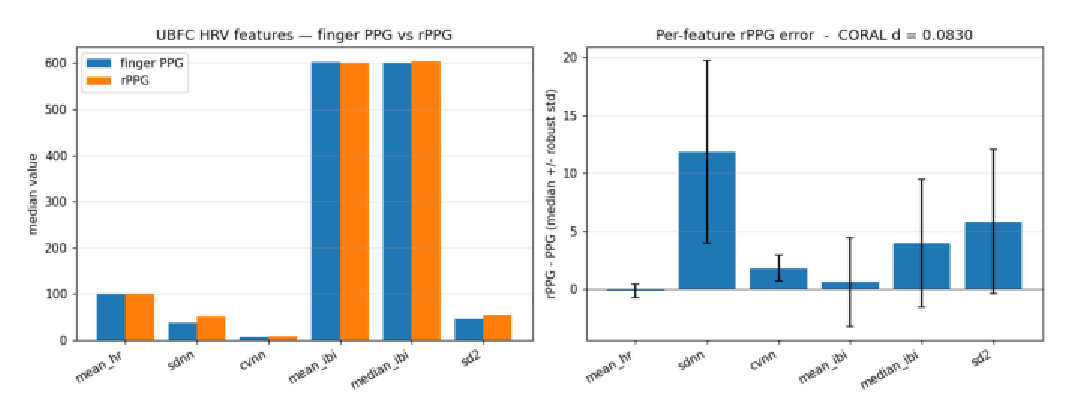
\includegraphics[width=\columnwidth]{figures/modality_gap.pdf}
\caption{Per-feature rPPG error on UBFC ($n{=}42$). Left: median
values from finger PPG and rPPG. Right: median deviations (bars) with
MAD-scaled standard deviations (whiskers). Six retained features.}
\label{fig:modality-gap}
\end{figure}

\subsection{Cross-modal stress adaptation}
Table~\ref{tab:stress} reports the five configurations on both binary
and 3-class tasks. The pattern is monotonic on both:
source-only $>$ jitter $>$ bridge $>$ full CMHT, with wrist-only as
the second-worst configuration on both tasks.

\begin{table}[t]
\caption{Stress classification (subject-independent, 5-seed
mean $\pm$ std). Per-subject macro-F1 ($n{=}15$). Wilcoxon $p$
values compare against source-only.}
\label{tab:stress}
\centering
\small
\begin{tabular}{lcccc}
\toprule
\multirow{2}{*}{Method} & \multicolumn{2}{c}{Binary} &
\multicolumn{2}{c}{3-class} \\
\cmidrule(lr){2-3} \cmidrule(lr){4-5}
 & F1 & $p$ & F1 & $p$ \\
\midrule
source\_only   & $\mathbf{0.759 \pm 0.236}$ & ---    & $\mathbf{0.457 \pm 0.162}$ & --- \\
jitter\_only   & $0.730 \pm 0.237$         & $0.028$ & $0.445 \pm 0.148$ & $0.330$ \\
wrist\_only    & $0.646 \pm 0.265$         & $0.073$ & $0.340 \pm 0.167$ & $0.095$ \\
bridge\_only   & $0.683 \pm 0.251$         & $0.221$ & $0.365 \pm 0.208$ & $0.151$ \\
full\_cmht     & $0.627 \pm 0.172$         & $0.083$ & $0.401 \pm 0.114$ & $0.151$ \\
\bottomrule
\end{tabular}
\end{table}

The wrist-only result is central: identical subjects, identical labels,
identical feature vector, differing only in the sensor used for
training. Chest ECG features yield $0.759$ binary F1; wrist PPG yields
$0.646$. The $(0.11)$ gap is a property of the two contact modalities,
not of any adaptation method. All alignment strategies that push
features toward the PPG space inherit a fraction of this gap.

\subsection{Emotion classification}
On the 3-class AffectNet valence task, EfficientNet-B0 reaches
$0.740$ accuracy, $0.713$ macro-F1, $0.738$ balanced accuracy, and
$0.593$ Cohen's $\kappa$. Per-class F1 is $0.87$ positive, $0.56$
neutral, $0.71$ negative. The neutral class is limited by annotation
ambiguity in AffectNet.

% ======================================================================
\section{Discussion}

The paper's central claim is narrow: \emph{covariance alignment from
chest ECG to wrist PPG (or rPPG) HRV features does not improve
subject-independent stress classification on WESAD, and the reason is
that the target modality is less stress-discriminative than the
source.}

Two observations support this. First, source-only and wrist-only
classifiers use the same subject set, labels, and feature vector; the
only difference is the sensor. The consistent $\sim 0.10$ F1 gap
between them is therefore attributable to the modality, not the
classifier. Second, every alignment method that interpolates toward
the PPG space moves features in the direction of this gap. On both
task difficulties, this produces a monotonic degradation.

The finding reframes a common assumption. Prior work implicitly
treats sensing modality as a nuisance variable that adaptation can
neutralize. Our measurements suggest that for HRV-based stress
detection, modality is signal: the choice of sensor changes what the
classifier can learn, and no covariance matching recovers the missing
information.

We emphasize what we do \emph{not} claim. We do not claim that all
domain adaptation fails, that DANN or MMD would behave identically,
or that our synthetic target is a substitute for real stress-labelled
video. Our claim is bounded by the specific methods, features, and
dataset we evaluated.

% ======================================================================
\section{Limitations}

\textbf{Datasets.} WESAD contains 15 subjects, which limits statistical
power. UBFC clips are $\sim$50 seconds, too short for reliable
frequency-domain HRV. AffectNet is used as a 7{,}797-image subset
(1.7\% of the full corpus).

\textbf{Synthetic target.} The synthetic-rPPG WESAD is constructed
from a measured noise model applied to contact features. It is a
calibrated proxy, not a stress-labelled video dataset. A prospective
validation with UBFC-Phys~\cite{meziati2021} is left for future work.

\textbf{Classical rPPG.} HR extraction uses POS without any learned
component. A deep rPPG baseline (MTTS-CAN, PhysNet) is not evaluated.

\textbf{Emotion module.} The emotion head is trained on a small
AffectNet subset and is not connected to the stress argument. It is
included as a demonstration of a second input modality.

\textbf{Fairness.} rPPG performance varies with skin tone, lighting,
and motion. Neither WESAD nor UBFC is demographically diverse. No
subgroup analysis is performed.

\textbf{Deployment.} No mobile or edge deployment is evaluated.
Latency, memory, and on-device performance are not reported.

% ======================================================================
\section{Ethics and Privacy}

Contactless stress detection from facial video raises privacy and
misuse concerns. Video-based physiological measurement can infer
affective state without active cooperation. We recommend explicit
per-session consent for any such system, on-device processing where
possible to avoid transmitting raw video, no retention of raw video
after feature extraction, and prohibition of use in employment,
insurance, or law-enforcement contexts without independent ethical
review. All datasets are used under their original research licenses;
no human subject data was collected for this work.

% ======================================================================
\section{Conclusion}

We presented a contactless wellness pipeline with HR, HRV, stress, and
emotion modules, validated at 2.71 bpm HR MAE on 42 UBFC subjects and
0.74 emotion accuracy on a 3-class AffectNet subset. We then studied
HRV cross-modal adaptation and found that chest-ECG features are
systematically more stress-discriminative than wrist-PPG features on
the same subjects, and that aligning toward the PPG space degrades
classification monotonically. We report this as a measured observation
about modality-specific discriminability. Future work should focus on
population-level and modality-aware adaptation strategies, and on
evaluating whether the discriminability gap persists in prospective
contactless stress datasets.

\section*{Reproducibility}

Code, cached features, and trained model weights are released at
\url{[GitHub URL]}. All experiments reproduce from public datasets
(WESAD, UBFC-rPPG, AffectNet) in under four hours on a single laptop.

% ======================================================================
\begin{thebibliography}{00}
\bibitem{verkruysse2008} W. Verkruysse, L. O. Svaasand, and J. S. Nelson,
``Remote plethysmographic imaging using ambient light,''
\emph{Opt. Express}, vol. 16, no. 26, pp. 21434--21445, 2008.

\bibitem{dehaan2013} G. de Haan and V. Jeanne, ``Robust pulse rate
from chrominance-based rPPG,'' \emph{IEEE Trans. Biomed. Eng.},
vol. 60, no. 10, pp. 2878--2886, 2013.

\bibitem{wang2017} W. Wang et al., ``Algorithmic principles of remote
PPG,'' \emph{IEEE Trans. Biomed. Eng.}, vol. 64, no. 7,
pp. 1479--1491, 2017.

\bibitem{mcduff2017} D. McDuff, S. Gontarek, and R. Picard,
``Improvements in remote cardiopulmonary measurement using a
five-band digital camera,'' \emph{IEEE Trans. Biomed. Eng.},
vol. 61, no. 10, pp. 2593--2601, 2014.

\bibitem{yan2019} B. P. Yan et al., ``Resting and postexercise heart
rate variability determined by contact and non-contact
photoplethysmography,'' \emph{J. Electrocardiol.}, vol. 57,
pp. S18--S24, 2019.

\bibitem{meziati2021} R. Meziati Sabour et al., ``UBFC-Phys: A
multimodal database for psychophysiological studies of social
stress,'' \emph{IEEE Trans. Affective Computing}, vol. 14, no. 1,
pp. 23--37, 2023.

\bibitem{schmidt2018} P. Schmidt, A. Reiss, R. Duerichen, C. Marberger,
and K. Van Laerhoven, ``Introducing WESAD, a multimodal dataset for
wearable stress and affect detection,'' in \emph{Proc. ICMI}, 2018.

\bibitem{koelstra2012} S. Koelstra et al., ``DEAP: A database for
emotion analysis using physiological signals,''
\emph{IEEE Trans. Affective Computing}, vol. 3, no. 1, pp. 18--31,
2012.

\bibitem{sun2016} B. Sun, J. Feng, and K. Saenko, ``Return of
frustratingly easy domain adaptation,'' in \emph{Proc. AAAI}, 2016.

\bibitem{ganin2016} Y. Ganin et al., ``Domain-adversarial training of
neural networks,'' \emph{JMLR}, vol. 17, no. 59, pp. 1--35, 2016.

\bibitem{bobbia2019} S. Bobbia, R. Macwan, Y. Benezeth, A. Mansouri,
and J. Dubois, ``Unsupervised skin tissue segmentation for remote
photoplethysmography,'' \emph{Pattern Recognit. Lett.}, vol. 124,
pp. 82--90, 2019.

\bibitem{mollahosseini2019} A. Mollahosseini, B. Hasani, and
M. H. Mahoor, ``AffectNet: A database for facial expression, valence,
and arousal computing in the wild,'' \emph{IEEE Trans. Affective
Computing}, vol. 10, no. 1, pp. 18--31, 2019.

\end{thebibliography}

\end{document}